\chapter{Investigating the Design of new CIPRNGs}
\label{CI dev}
\minitoc

In this chapter, firstly the CIPRNG methods have been verified an optimization technique improving the statistical performance for large varieties of pseudorandom generators. Then some formerly proposed researches on CIPRNGs versions 1 and 2 are deepened, the designs of our two brand new versions of discrete chaotic iterations based pseudorandom number generators, satisfying Devaney's chaos, are proposed and discussed. Detail operations of the proposed approach are described in this chapter, while their performance and  comparative studies will be presented in a next one. The works presented in this chapter have been formerly published in \cite{submit2,bfg12a:ip} and submitted in \cite{submit1, submit3}.

\section{An optimization technique on pseudorandom generators based on chaotic iterations}
In this section, the behavior of our previous CIPRNG versions regarding 
the statistics of the inputted generators are carried out systematically, and the results are discussed.
Here, CIPRNG Version 1, Version 2 and XOR CIPRNG method are applied to experimented.
Indeed PRNGs are often based on modular arithmetic, logical operations like bitwise exclusive or (XOR), and on circular shifts of bit vectors.
However the security level of some PRNGs of this kind has been revealed inadequate by today's standards.
Since different biased generators can possibly have their own side effects when inputted into our mixed generators, it is normal to enlarge the set of tested inputted PRNGs, to determine if the observed improvement still remains.
We will thus show in this chapter that the intended statistical improvement is really effective for all of these most famous generators. To be notice, we have formally published the works in \cite{bfg12a:ip}.

\subsection{PRNGs tested}
Knowing that there is no universal generator, it is strongly recommended to test a stochastic application with a large set of different PRNGs~\cite{DavidRC2003643}.Such generators should cover the four major classes: linear generators, lagged generators, inversive generators, and mix generators (described in Chapter~\ref{Review of works}). Here ten PRNGs from Chapter~\ref{Review of works} would be applied in the experiment: LCG, MRG from type Linear PRNGs; AWC, SWB, SWC, and GFSR from type Lagged PRNGs; INV from type ICG PRNGs; Lastly the combination of two LCGs (namely 2LCG), three LCGs (namely 3LCG), and two MRGs(namely 2MRG) from type Mixed PRNGs. 

For instance, inversive generators are very interesting for verifying simulation results obtained with a linear congruential generator (LCG),
because their internal structure and correlation behavior strongly differ from what LCGs produce.
Since these generators have revealed several issues, some scientists refrain from using them.
In what follows, chaotic properties will be added to these PRNGs, leading to noticeable improvements observed by statistical tests.

A theoretical proof for the randomness of a generator is impossible to give, therefore statistical inference based on observed sample sequences produced by the generator seems to be the best option.
Considering the properties of binary random sequences, various statistical tests can be designed to evaluate the assertion that the sequence is generated by a perfectly random source. We have performed some statistical tests for the CIPRNGs proposed here. These tests include NIST suite~\cite{ANDREW2008} and DieHARD battery of tests~\cite{Marsaglia1996}.

\subsection{Results of PRNGs}
\label{Results and discussion}

\begin{sidewaystable}
\caption{NIST and DieHARD tests suite passing rates for PRNGs without CI}
\label{NIST and DieHARD tests suite passing rate the for PRNGs without CI}
\centering
\begin{tabular}{|l||c|c|c|c|c|c|c|c|c|c|}
    \hline\hline
Types of PRNGs & \multicolumn{2}{c|}{Linear PRNGs} & \multicolumn{4}{c|}{Lagged PRNGs} & \multicolumn{1}{c|}{ICG PRNGs} & \multicolumn{3}{c|}{Mixed PRNGs}\\ \hline
\backslashbox{\textbf{$Tests$}} {\textbf{$PRNG$}} & LCG& MRG& AWC & SWB  & SWC & GFSR & INV & LCG2& LCG3& MRG2 \\ \hline
NIST & 11/15 & 14/15 &\textbf{15/15} & \textbf{15/15}   & 14/15 & 14/15  & 14/15 & 14/15& 14/15& 14/15 \\ \hline
DieHARD & 16/18 & 16/18 & 15/18 & 16/18 & \textbf{18/18} & 16/18 & 16/18 & 16/18& 16/18& 16/18\\ \hline
\end{tabular}
\end{sidewaystable}



Table~\ref{NIST and DieHARD tests suite passing rate the for PRNGs without CI} shows the results on the batteries recalled in a
previous chapter, indicating that almost all the PRNGs introduced here cannot pass all their embedding tests. In other words, the statistical quality of these PRNGs cannot fulfill the up-to-date standards presented previously. We will show that the CIPRNG can solve this issue.

To illustrate the effects of this CIPRNG in detail, experiments will be divided in three parts:
\begin{enumerate}
  \item \textbf{Single CIPRNG}: The PRNGs involved into the chaotic iterations computing are of the same category.
  \item \textbf{Mixed CIPRNG}: Two different types of generators are mixed during the CIPRNG process.
  \item \textbf{Multiple CIPRNG}: The generator is obtained by repeating the composition of the iteration function as follows: $x^0\in \mathds{B}^{\mathsf{N}}$, and $\forall n\in \mathds{N}^{\ast },\forall i\in \llbracket1;\mathsf{N}\rrbracket,$
\begin{equation}
\begin{array}{l}
x_i^n=\left\{
\begin{array}{l}
x_i^{n-1}~~~~~\text{if}~S^n\neq i \\
\forall j\in \llbracket1;\mathsf{m}\rrbracket,f^m(x^{n-1})_{S^{nm+j}}~\text{if}~S^{nm+j}=i.\end{array} \right. \end{array}
\end{equation}
$m$ is called the \emph{functional power}.
\end{enumerate}


We have performed statistical analysis of each of the aforementioned CIPRNGs.
The results are reproduced in Tab.~\ref{NIST and DieHARD tests suite passing rate the for PRNGs without CI} and \ref{NIST and DieHARD tests suite passing rate the for single CIPRNGs}.
The scores written in boldface indicate that all the tests have been passed successfully, whereas an asterisk ``*'' means that the considered passing rate has been improved.
\subsection{Tests based on the Single CIPRNG}

\begin{sidewaystable}
\renewcommand{\arraystretch}{1.3}
\caption{NIST and DieHARD tests suite passing rates for PRNGs with CI}
\label{NIST and DieHARD tests suite passing rate the for single CIPRNGs}
\centering
  \begin{tabular}{|l||c|c|c|c|c|c|c|c|c|c|c|c|}
    \hline
Types of PRNGs & \multicolumn{2}{c|}{Linear PRNGs} & \multicolumn{4}{c|}{Lagged PRNGs} & \multicolumn{1}{c|}{ICG PRNGs} & \multicolumn{3}{c|}{Mixed PRNGs}\\ \hline
\backslashbox{\textbf{$Tests$}} {\textbf{$Single~CIPRNG$}} & LCG  & MRG & AWC & SWB & SWC & GFSR & INV& LCG2 & LCG3& MRG2 \\ \hline\hline
Version 1 CIPRNG\\ \hline \hline
NIST & \textbf{15/15} *  & \textbf{15/15} * & \textbf{15/15}   & \textbf{15/15}   & \textbf{15/15} * & \textbf{15/15} * & \textbf{15/15} *& \textbf{15/15} * & \textbf{15/15} * & \textbf{15/15} \\ \hline
DieHARD & \textbf{18/18} *  & \textbf{18/18} * & \textbf{18/18} *  & \textbf{18/18} *  & \textbf{18/18}  & \textbf{18/18} * & \textbf{18/18} *& \textbf{18/18} * & \textbf{18/18} *& \textbf{18/18} * \\ \hline
Version 2 CIPRNG\\ \hline \hline
NIST & \textbf{15/15} *  & \textbf{15/15} * & \textbf{15/15}   & \textbf{15/15}  & \textbf{15/15} * & \textbf{15/15} * & \textbf{15/15} *& \textbf{15/15} * & \textbf{15/15} * & \textbf{15/15} \\ \hline
DieHARD & \textbf{18/18} *  & \textbf{18/18} * & \textbf{18/18} * & \textbf{18/18} * & \textbf{18/18}  & \textbf{18/18} * & \textbf{18/18} * & \textbf{18/18} * & \textbf{18/18} *& \textbf{18/18} *\\ \hline
Xor CIPRNG\\ \hline\hline
NIST & 14/15*& \textbf{15/15} *   & \textbf{15/15}   & \textbf{15/15}   & 14/15 & \textbf{15/15} * & 14/15& \textbf{15/15} * & \textbf{15/15} *& \textbf{15/15}  \\ \hline
DieHARD & 16/18 & 16/18 & 17/18* & \textbf{18/18} * & \textbf{18/18}  & \textbf{18/18} * & 16/18 & 16/18 & 16/18& 16/18\\ \hline
\end{tabular}
\end{sidewaystable}

The statistical tests results of the PRNGs using the single CIPRNG method are given in Tab.~\ref{NIST and DieHARD tests suite passing rate the for single CIPRNGs}.
We can observe that, except for the Xor CIPRNG, all of the CIPRNGs have passed the 15 tests of the NIST battery and the 18 tests of the DieHARD one.
Moreover, considering these scores, we can deduce that both the single Version 1 CIPRNG and the single Version 2 CIPRNG are relatively steadier than the single Xor CIPRNG approach, when applying them to different PRNGs.
However, the Xor CIPRNG is obviously the fastest approach to generate a CI random sequence, and it still improves the statistical properties relative to each generator taken alone, although the test values are not as good as desired.

Therefore, all of these three ways are interesting, for different reasons, in the production of pseudorandom numbers and,
on the whole, the single CIPRNG method can be considered to adapt to or improve all kinds of PRNGs.

To have a realization of the Xor CIPRNG that can pass all the tests embedded into the NIST battery, the Xor CIPRNG with multiple functional powers are investigated in Section~\ref{Tests based on Multiple CIPRNG}.



\subsection{Tests based on the Mixed CIPRNG}

To compare the previous approach with the CIPRNG design that uses a Mixed CIPRNG, we have taken into account the same inputted generators than in the previous section.
These inputted couples $(PRNG_1,PRNG_2)$ of PRNGs are used in the Mixed approach as follows:
\begin{equation}
\left\{
\begin{array}{l}
x^0 \in \llbracket 0, 2^\mathsf{N}-1 \rrbracket, S \in \llbracket 0, 2^\mathsf{N}-1 \rrbracket^\mathds{N} \\
\forall n \in \mathds{N}^*, x^n = x^{n-1} \oplus PRNG_1\oplus PRNG_2,
\end{array}
\right.
\label{equation Oplus}
\end{equation}

With this Mixed CIPRNG approach, both the Version 1 CIPRNG and Version 2 CIPRNG continue to pass all the NIST and DieHARD suites.
In addition, we can see that the PRNGs using a Xor CIPRNG approach can pass more tests than previously.
The main reason of this success is that the Mixed Xor CIPRNG has a longer period.
Indeed, let $n_{P}$ be the period of a PRNG $P$, then the period deduced from the single Xor CIPRNG approach is obviously equal to:
\begin{equation}
n_{SXORCI}=
\left\{
\begin{array}{ll}
n_{P}&\text{if~}x^0=x^{n_{P}}\\
2n_{P}&\text{if~}x^0\neq x^{n_{P}}.\\
\end{array}
\right.
\label{equation Oplus}
\end{equation}

Let us now denote by $n_{P1}$ and $n_{P2}$ the periods of respectively the $PRNG_1$ and $PRNG_2$ generators, then the period of the Mixed Xor CIPRNG will be:
\begin{equation}
n_{XXORCI}=
\left\{
\begin{array}{ll}
LCM(n_{P1},n_{P2})&\text{if~}x^0=x^{LCM(n_{P1},n_{P2})}\\
2LCM(n_{P1},n_{P2})&\text{if~}x^0\neq x^{LCM(n_{P1},n_{P2})}.\\
\end{array}
\right.
\label{equation Oplus}
\end{equation}

In Tab.~\ref{DieHARD fail mixex CIPRNG}, we only show the results for the Mixed CIPRNGs that cannot pass all DieHARD suites (the NIST tests are all passed). It demonstrates that Mixed Xor CIPRNG involving LCG, MRG, LCG2, LCG3, MRG2, or INV cannot pass the two following tests, namely the ``Matrix Rank 32x32'' and the ``COUNT-THE-1's'' tests contained into the DieHARD battery. Let us recall their definitions:

\begin{itemize}
 \item \textbf{Matrix Rank 32x32.} A random 32x32 binary matrix is formed, each row having a 32-bit random vector. Its rank is an integer that ranges from 0 to 32. Ranks less than 29 must be rare, and their occurences must be pooled with those of rank 29. To achieve the test, ranks of 40,000 such random matrices are obtained, and a chisquare test is performed on counts for ranks 32,31,30 and for ranks $\leq29$.

 \item \textbf{COUNT-THE-1's TEST} Consider the file under test as a stream of bytes (four per  2 bit integer).  Each byte can contain from 0 to 8 1's, with probabilities 1,8,28,56,70,56,28,8,1 over 256.  Now let the stream of bytes provide a string of overlapping  5-letter words, each ``letter'' taking values A,B,C,D,E. The letters are determined by the number of 1's in a byte: 0,1, or 2 yield A, 3 yields B, 4 yields C, 5 yields D and 6,7, or 8 yield E. Thus we have a monkey at a typewriter hitting five keys with various probabilities (37,56,70,56,37 over 256).  There are $5^5$ possible 5-letter words, and from a string of 256,000 (over-lapping) 5-letter words, counts are made on the frequencies for each word.   The quadratic form in the weak inverse of the covariance matrix of the cell counts provides a chisquare test: Q5-Q4, the difference of the naive Pearson sums of $(OBS-EXP)^2/EXP$ on counts for 5- and 4-letter cell counts.
\end{itemize}

The reason of these fails is that the output of LCG, LCG2, LCG3, MRG, and MRG2 under the experiments are in 31-bit. Compare with the Single CIPRNG, using different PRNGs to build CIPRNG seems more efficient in improving random number quality (mixed Xor CI can 100\% pass NIST, but single cannot).

\begin{table*}
\renewcommand{\arraystretch}{1.3}
\caption{Scores of mixed Xor CIPRNGs when considering the DieHARD battery}
\label{DieHARD fail mixex CIPRNG}
\centering
  \begin{tabular}{|l||c|c|c|c|c|c|}
    \hline
\backslashbox{\textbf{$PRNG_1$}} {\textbf{$PRNG_0$}} & LCG & MRG & INV & LCG2 & LCG3 & MRG2 \\ \hline\hline
LCG  &\backslashbox{} {} &16/18&16/18 &16/18 &16/18 &16/18\\ \hline
MRG &16/18 &\backslashbox{} {} &16/18&16/18 &16/18  &16/18\\ \hline
INV &16/18 &16/18&\backslashbox{} {} &16/18 &16/18&16/18    \\ \hline
LCG2  &16/18 &16/18 &16/18 &\backslashbox{} {}  &16/18&16/18\\ \hline
LCG3  &16/18 &16/18 &16/18&16/18&\backslashbox{} {} &16/18\\ \hline
MRG2 &16/18  &16/18 &16/18&16/18 &16/18 &\backslashbox{} {}  \\ \hline
\end{tabular}
\end{table*}

\subsection{Tests based on the Multiple CIPRNG}
\label{Tests based on Multiple CIPRNG}

Until now, the combination of at most two input PRNGs has been investigated.
We now regard the possibility to use a larger number of generators to improve the statistics 
of the generated pseudorandom numbers, leading to the multiple functional power approach.
For the CIPRNGs which have already pass both the NIST and DieHARD suites with 2 inputted PRNGs 
(all the Old and Version 2 CIPRNGs, and some of the Xor CIPRNGs), it is not meaningful to consider 
their adaption of this multiple CIPRNG method, hence only the Multiple Xor CIPRNGs, 
having the following form, will be investigated.
\begin{equation}
\left\{
\begin{array}{l}
x^0 \in \llbracket 0, 2^\mathsf{N}-1 \rrbracket, S \in \llbracket 0, 2^\mathsf{N}-1 \rrbracket^\mathds{N} \\
\forall n \in \mathds{N}^*, x^n = x^{n-1} \oplus S^{nm}\oplus S^{nm+1}\ldots \oplus S^{nm+m-1} ,
\end{array}
\right.
\label{equation Oplus}
\end{equation}

The question is now to determine the value of the threshold $m$ (the functional power) making 
the multiple CIPRNG being able to pass the whole NIST battery.
Such a question is answered in Tab.~\ref{threshold}.


\begin{table*}
\renewcommand{\arraystretch}{1.3}
\caption{Functional power $m$ making it possible to pass the whole NIST battery}
\label{threshold}
\centering
  \begin{tabular}{|l||c|c|c|c|c|c|c|c|}
    \hline
Inputted $PRNG$ & LCG & MRG & SWC & GFSR & INV& LCG2 & LCG3  & MRG2 \\ \hline\hline
Threshold  value $m$& 19 & 7  & 2& 1 & 11& 9& 3& 4\\ \hline\hline
\end{tabular}
\end{table*}

\subsection{Results Summary}

We can summarize the obtained results as follows.
\begin{enumerate}
\item The CIPRNG method is able to improve the statistical properties of a large variety of PRNGs.
\item Using different PRNGs in the CIPRNG approach is better than considering several instances of one unique PRNG.
\item The statistical quality of the outputs increases with the functional power $m$.
\end{enumerate}

In this chapter, we first have formalized the CI methods that has been already presented in previous research articles.
These CI methods are based on iterations that have been topologically proven as chaotic.
Then 10 usual PRNGs covering all kinds of generators have been applied, and the NIST and DieHARD batteries have been tested.
Analyses show that PRNGs using the CIPRNG methods have improvements of their statistics.
CIPRNG techniques should be considered as post-treatments on pseudorandom number generators to improve both their randomness and security.


\section{``LUT'' CIPRNG(XORshift,XORshift) Version 3}
\label{LUT CI(XORshift,XORshift) algorithms and example}
\subsection{Introduction}

The LUT (Lookup-Table) CIPRNG version 3 is an improved version of the CIPRNG version 2. The key-ideas are:
\begin{enumerate}
\item To use a Lookup Table for a faster generation of strategies. 
These strategies satisfy the same property than the ones provided by the decimation process.
\item And to use all the bits provided by the two inputted generators (to discard none of them).
\end{enumerate}
%Before putting these key-ideas together, we can make a first practical remark in order to improve the speed of all of our generators.
These key-ideas are put together by the following way.

%In the LUT version of the proposed generator, chaotic iterations are realized as in the Version 2 CIPRNG, in order to generate a sequence $\left(x^n\right)_{n\in\mathds{N}} \in \left(\mathds{B}^N\right)^\mathds{N}$ of Boolean vectors ($N \in \mathds{N}^*, N \geqslant 2$).
Let us firstly recall that in chaotic iterations, only the cells designed by $S^{n}-$th are ``iterated'' 
at the $n^{th}$ iteration.
$S^n$ can be either a component (\emph{i.e.}, only one cell is updated at each iteration, 
so $S^n \in \llbracket 1;N \rrbracket$) or a subset of components (any number of cells can be 
updated at each iteration, that is, $S^n \subset \llbracket 1;N \rrbracket$).
The first kind of strategies are called ``unary strategies'' whereas the second one are denoted by ``general strategies''.
In the last case, each term $S^n$ of the strategy can be represented by an integer lower than $2^N$, 
designed by $\mathcal{S}^n$, for a system having $N$ bits: the $k^{th}$ component of the system is 
updated at iteration number $n$ if and only if the $k^{th}$ digit of the binary decomposition of $\mathcal{S}^n$ is 1.
For instance, let us consider that $\mathcal{S}^n=5$, and that we iterate on a system having 6 bits ($N=6$).
As the integer 5 has a binary decomposition equal to 000101, we thus conclude that the cells number 1 and 3 
will be updated when the system changes its state from $x^{n}$ to $x^{n+1}$.
In other words, in that situation, $\mathcal{S}^n=5 \in \llbracket 0,2^6-1\rrbracket \Leftrightarrow 
S^n = \{1, 3\} \subset \llbracket 1, 6 \rrbracket$.
To sum up, to provide a general strategy of $\llbracket 1;N \rrbracket$ is equivalent to 
give an unary strategy in $\llbracket 0; 2^N-1 \rrbracket$.
Let us now take into account this remark.

Until now the proposed generators have been presented in this document by using unary 
strategies (obtained by the inputted PRNG2) that are finally grouped by ``packages'' 
(the size of these packages is given by the generator PRNG1 $m$): after having used each terms 
in the current package $S^{m^n},...,S^{m^{n+1}-1}$, the current state of the system is published as an output.
Obviously, when considering the CIPRNG version 2, these packages of unary strategies defined by the 
couple $(S,m)\in \llbracket 1;N \rrbracket \times \llbracket 0;N \rrbracket$ correspond to 
subsets of $\llbracket 1;N \rrbracket$ having the form $\left\{S^{m^n},...,S^{m^{n+1}-1}\right\}$, 
which are general strategies.
As stated before, these lasts can be rewritten as unary strategies that can 
be described as sequences in $\llbracket 0; 2^N-1 \rrbracket$.



The advantage of such an equivalence is to reduce the complexity of the proposed PRNG.
Indeed the LUT CIPRNG($S$,$m$) can be written as:
\begin{equation}
x^n = x^{n-1} \oplus \mathcal{S}^n.
\end{equation}
where $\mathcal{S}$ is the unary strategy (in $\llbracket 0; 2^N-1 \rrbracket$) associated 
to the couple $(S,m)\in \llbracket 1;N \rrbracket \times \llbracket 0,N \rrbracket$.

The speed improvement is obvious, the sole issue is to understand how to change $(S,m)$ by $\mathcal{S}$.
The problem to consider is that all the sequences of $\llbracket 0; 2^n-1 \rrbracket$ are not convenient.
Indeed, the properties required for the couple $(S,m)$ ($S$ must not be uniformly distributed, 
and a cell cannot be changed twice between two outputs) must be translated in requirements for 
$\mathcal{S}$ if we want to satisfy both speed and randomness.
Such constrains are solved by working on the sequence $m$ and by using some well-defined Lookup 
Tables presented in the following sections.

\subsection{Sequence $m$}
\label{LUT1}

In order to improve the speed of the proposed generator, 
the first plan is to take the best usage of the bits generated by the inputted PRNGs.
The problem is that the PRNG generating the integers of $m^n$ does not necessary takes its values 
into $\llbracket 0, N \rrbracket$, where $N$ is the size of the system.

For instance, in the CIPRNG version 2 presented previously, assume that this sequence is obtained by a $32-$bit word
XORshift, which produces integers belonging into $\llbracket 0, 2^{32}-1 \rrbracket$.
However, the iterated system has 4 cells ($N=4$) in the example proposed previously thus, 
to define the sequence $m^n$, we compute the remainder modulo 4 of each integer provided by the XORshift generator.
In other words, only the last 4 bits of each 32 bits vector generated by the second XORshift are used.
Obviously this stage can be easily optimized, by splitting this 32-bits vector into 8 subsequences of 4 bits.
Thus, for example, a call of $32$-bit output word XORshift() will now generate $8$ terms of the sequence $m$, instead of only one term in the former generator.

This common-sense action can be easily generalized to any size $N \leqslant 32$ of 
the system by the procedure described in Algo.\ref{b fuction}. The idea is simply 
to make a shift of the binary vector $a$ produced by the XORshift generator, by $0$, $N$, $2N$,... 
bits to the right, depending on the remainder $c$ of $n$ modulo $\lfloor N/32 \rfloor$ (that is, 
$a \gg (N \times c)$), and to take the bits between the positions $32-N$ and $32$ of this vector 
(corresponding to the right part ``$\& (2^N-1)$'' of the formula).
In that situation, all the bits provided by a PRNG1 are used when $N$ divides 32.

\begin{algorithm}
\begin{algorithmic}[1]
\STATE $c=n~mod~\lfloor32/N\rfloor$
\IF {$c=0$}
  \STATE $a = PRNG1()$
\ENDIF

  \STATE $b^n= (a\gg (N \times c))\& (2^N-1)$
\STATE Return {$b^n$}
\medskip
\end{algorithmic}
\caption{Generation of sequence $b^n$}
\label{b fuction}
\end{algorithm}

This Algo.\ref{b fuction} produces a sequence $(b^n)_{n \in \mathds{N}}$ of integers belonging into 
$\llbracket 0, 2^N-1 \rrbracket$.
It is now possible to define the sequence $m$ by adapting the Eq.(\ref{v2_g2}) or 
Eq.(\ref{v2_g1}) of CIPRNG2 version 2 as follows.

\begin{equation}
\label{lut_m}
m^n = f(b^n)=
\left\{
\begin{array}{l}
0 \text{ if }0				\leqslant {b^n} < {C^0_N},\\
1 \text{ if }{C^0_N}	\leqslant {b^n} < \sum_{i=0}^1 {C^i_N},\\
2 \text{ if }\sum_{i=0}^1{C^i_N}	\leqslant {b^n} < \sum_{i=0}^2 {C^i_N},\\
\vdots~~~~~					~~\vdots~~~		    ~~~~\\
N \text{ if }\sum_{i=0}^{N-1} {C^i_N}	\leqslant {b^n} < 2^N.\\
\end{array}
\right.
\end{equation}

This common-sense measure can be improved another time if $N$ is not very large by using the first Lookup 
Table of this document, which is called LUT-1.
This improvement will be firstly explained through an example.

Let us consider that $N=4$, so the sequence $(b^n)_{n \in \mathds{N}}$ belongs into $\llbracket 0, 15 \rrbracket$.
The function $f$ of Eq.(\ref{lut_m}) must translate each $b^n$ into an integer $m^n \in \llbracket 0,4 \rrbracket$, 
in such a way that the non-uniformity exposed previously is respected.
Instead of defining the function $f$ analytically, a table can be given containing all the images 
of the integers into $\llbracket 0, 15 \rrbracket$ (see Tab.\ref{LUT1 for example} for instance).
As stated before, the frequencies of occurrence of the images 0,1,2, 3, and 4 must be respectively equal 
to $\frac{C_4^0}{2^4}$, $\frac{C_4^1}{2^4}$, $\frac{C_4^2}{2^4}$, $\frac{C_4^3}{2^4}$, and $\frac{C_4^4}{2^4}$.
This requirement is equivalent to demand $C_N^i$ times the number $i$, which can be translated in terms of permutations.
For instance, when $N=4$, any permutation of the list [0,1,1,1,1,2,2,2,2,2,2,3,3,3,3,4] is convenient to 
define the image of [0,1,2,...,14,15] by $f$.

This improvement is implemented in Algo.\ref{LUT1 creation}, 
which returns a table $lut1$ such that $m^n=lut1[b^n]$.

\begin{algorithm}
\caption{The LUT-1 table generation}\label{LUT1 creation}
\begin{algorithmic}[1]
\STATE $i=0$
    \FOR{$j=0...N$}
        \WHILE{$i<C_N^j$}
             \STATE $lut1[i]=j$
             \STATE $i = i + 1$
         \ENDWHILE
    \ENDFOR
\STATE Return $lut1$
\end{algorithmic}
\end{algorithm}

\begin{table*} 
\renewcommand{\arraystretch}{1.3}
\caption{A LUT-1 table for $N=4$}
\label{LUT1 for example}
\centering
  \begin{tabular}{|c|c|c|c|c|c|c|c|c|c|c|c|c|c|c|c|c|c|}
    \hline
 $b^n$  & 0 & 1 & 2 & 3 & 4 & 5 & 6 & 7 &8 &9 &10 &11 &12 &13 &14 &15\\ \hline\hline
 $m^n$ & 0 & 1 & 1 & 1 & 1 & 2 & 2 & 2 & 2 & 2 & 2 & 3 & 3 &3 & 3 &4 \\ \hline

  \end{tabular}
\end{table*}


\subsection{Defining the strategy $\mathcal{S}$ with a LUT}
\label {LUT2}
The definition of the sequence $m$ allows to determine the number of cells 
that have to change between two outputs of the LUT CI generator.
There are $C_N^m$ possibilities to change $m$ bits in a vector of size $N$.
As we have to choose between these $C_N^m$ possibilities, we thus introduce the following sequence:
\begin{equation}
w^n=PRNG2()~mod~C^m_N.
\end{equation}

With this material it is now possible to define the lookup table that provides convenient strategies to the LUT CI generator.
If the size of the system is $N$, then this table has $N+1$ columns, numbered from $0$ to $N$.
The column number $m$ contains $C_N^m$ values.
All of these values have in common to present exactly $m$ times the digit $1$ 
and $N-m$ times the digit $0$ in their binary decomposition.
The order of appearance of these values in the column $m$ has no importance, 
the sole requirement is that no column contains a same integer twice.
Let us remark that this procedure leads to several possible LUTs.

\begin{algorithm}
\caption{$LUT21$ procedure}\label{LUT2_m creation}
\begin{algorithmic}[1]
\STATE Procedure~{LUT21}{($m,N,b,v,c$)}
\STATE $count\gets c$
\STATE $value\gets v$
 \IF {$count==M$}
    \STATE $lut2[M][num] = value$
    \STATE $num = num + 1$
  \ELSE
     \FOR {$i=b....N$}
     \STATE $value = value + 2^i$
     \STATE $count = count + 1$
     \STATE  Call {recurse LUT21}{($M,N,i+1,value,count$)}
     \STATE $value = v$
     \STATE $count = c$
   \ENDFOR
 \ENDIF
\STATE End Procedure
\end{algorithmic}
\end{algorithm}

An example of such a LUT is shown in Tab.\ref{LUT2 for example}, 
when Algo.\ref{LUT2 creation} gives a concrete procedure to obtain these tables.
This procedure makes recursive calls to the function $LUT21$ defined in Algo.\ref{LUT2_m creation}.
The $LUT21$ uses the following variables.
$b$ is used to avoid overlapping computations between two recursive calls, 
$v$ is to save the sum value between these calls, and $c$ counts the number of cells that have already been processed.
These parameters should be initialized as $0$.
For instance, the LUT presented in Tab.\ref{LUT2 for example} is 
the $lut2$ obtained in Algo.\ref{LUT2_m creation} and Algo.\ref{LUT2 creation} with $N=4$.


\begin{algorithm}
\caption{LUT-2 generation}\label{LUT2 creation}
\begin{algorithmic}[1]

 \FOR {$i=0....N$}
    \STATE Call {LUT21}{($i,N,0,0,0$)}
  \ENDFOR
\STATE Return lut2

\end{algorithmic}
\end{algorithm}



\begin{table} 
\renewcommand{\arraystretch}{1.3}
\caption{Example of a LUT for $N=4$}
\label{LUT2 for example}
\centering
  \begin{tabular}{|l||c|c|c|c|c|}\hline
\backslashbox{$w$}{$m$}
 & $m=0$ & $m=1$ & $m=2$ & $m=3$ & $m=4$ \\ \hline\hline
$w = 0$ & 0 & 1 & 3 & 7 & 15  \\ \hline
$w = 1$ &   & 2 & 5 & 11 &   \\ \hline
$w = 2$ &   & 4 & 6 & 13 & \\ \hline
$w = 3$ &   & 8 & 9 & 14 & \\ \hline
$w = 4$ &   &   & 10 &   & \\ \hline
$w = 5$ &   &   & 12 &   &  \\ \hline
  \end{tabular}
\end{table}



\subsection{LUT CI(XORshift,XORshift) Algorithm}
Here the CIPRNG version 3 (XORshift, XORshift) is proposed, two $32$-bit word XORshift generators are applied.
The LUT CI generator is defined by the following dynamical system:
\begin{equation}
x^n = x^{n-1} \oplus \mathcal{S}^n,
\end{equation}
where $x^O\in \llbracket 0,2^N-1\rrbracket$ is a seed and $\mathcal{S}^n = lut2[w^n][m^n] = lut2[w^n][lut1[b^n]]$, 
in which $b^n$ is provided by Algo.\ref{b fuction} and $w^n=XORshift2()~mod~C^m_N$.
An iteration of this generator is written in Algo.\ref{LUT CI algo}.
 \begin{algorithm}
 \caption{LUT CI algorithm}\label{LUT CI algo}
 \begin{algorithmic}[1]


  \STATE $b^n = PRNG1()$
    \STATE $m^n = lut1[b^n]$
    \STATE $w^n = PRNG2()$
    \STATE $S^n = lut2[m][w]$
    \STATE $x = x \oplus S^n$
    \STATE Return $x$

 \end{algorithmic}
 \end{algorithm}

\subsection{LUT CI(XORshift,XORshift) example of use}
In this example, $N = 4$ is chosen another time for easy understanding.
The initial state of the system $x^0$ can be seeded by the decimal part $t$ of the current time.
With the $t=484076$, then according to $t = t ~mod~ 16$, we have $x^0 = ( 0, 1, 0, 0)$ (or $x^0=4$).

Algo.\ref{LUT1 creation} provides the LUT-1 depicted in Tab.\ref{LUT1 for example}.
The first XORshift generator has returned $y = 0, 11, 7, 2, 10, 4, 1, 0, 3, 9,...$.
By using this LUT, we obtain $m = 0, 3, 2, 1, 2, 1, 1, 0, 1, 2,...$.
Then the Algo.\ref{LUT2 creation} is computed, leading to the LUT-2 given by Tab.\ref{LUT2 for example}.
So chaotic iterations of Algo.\ref{LUT CI algo} can be realized, 
to obtain in this example: 0100100101010001... or 4,9,5,1... As Tab.\ref{lut table application example} shows.

\begin{tiny}
\begin{table} 
\centering
\begin{tabular}{|c|c|c|c|c|}
\hline
$y$ &0 &11 &7&2 \\ \hline
$m$ &LUT-1[0]=0&LUT-1[11]=3&LUT-1[7]=2&LUT-1[2]=1  \\ \hline
$C_N^m$  & 1 & 4&6&4\\ \hline
$PRNG2~ mod~ C_N^m$  & 0 & 2 & 5 & 2\\ \hline
$S$  & LUT-2[0][0]=0& LUT-2[3][4]=13&LUT-2[2][5]=12&LUT-2[1][2]=4  \\ \hline
$x^{0}$ & $x^{0}$ &$x^{1}$ &$x^{2}$& $x^{3}$  \\
$0$ & $0$&$1$ & $0$& $0$\\
$1$ & $1$&$0$ & $1$& $0$\\
$0$ & $0$&$0$ & $0$& $0$ \\
$0$ & $0$&$1$ & $1$& $1$\\
\hline
\end{tabular}\\
\vspace{0.5cm}
Binary Output: $x_1^{0}x_2^{0}x_3^{0}x_4^{0}x_1^{1}x_2^{1}x_3^{1}x_4^{1}x_1^{2}x_2^{2}... = 0100100101010001...$\\
Integer Output:
$x^{0},x^{1},x^{2},x^{3}... = 4,11,8,1...$
\caption{Example of a LUT CI(XORshift,XORshift) generation}
\label{lut table application example}
\end{table}
\end{tiny}


\section{The version 4 category of CIPRNGs}
\subsection{CIPRNG version 4: the algorithm}

It is possible to add more complexity in updating the subset 
at each iteration
in Eq.~\ref{equation Oplus1} of XOR CI generator. 
When the updating function 
is the vectorial negation, this algorithm can be written as follows (Algo.\ref{new ci}):
\begin{algorithm}
\textbf{Input:} the internal state $x$ ($\mathsf{N}$ bits)\\
\textbf{Output:} a state $r$ of $\mathsf{N}$ bits
\begin{algorithmic}[1]
\FOR{$i=1,\dots,M$}
{
\STATE$S(i)= PRNG2\_i()$\;
}
\ENDFOR
\STATE$T = PRNG1()$\;
\STATE$r = x \oplus g_2(S(1),S(2),...~S(M))$,
\STATE return $r$\;
\medskip
\caption{An arbitrary round of the version 4 CI generator}
\label{new ci}
\end{algorithmic}
\end{algorithm}

$S(1), S(2), ..., S(M)$ are $M$ pseudorandom number sequences generated by $M$ XORshifts, $T^n$ is recommended to obtained by using a cryptographically secure
PRNG like the BBS. $(t_1^n,t_2^n,\dots,t_M^n)\in \{0,1\}^M$ is the binary representation of the $2^M$-bit number $T^n$.
Indeed, $(T^n)$ sequence's aim is to decimate
%A control sequence $T^n$ decimates 
the sequences %produced by the other generators 
$S(1),S(2),..., S(M)$, with a \emph{bitwise exclusive or} ($\oplus$), according to the following decimation rule:
\begin{itemize}
\item if $t^n_i = 0$, then $S^n(i)$ is discarded,
\item else $S^n(i)$ is kept for \emph{bitwise exclusive or} computing.
\end{itemize}
In brief, the produced output sequence $x^n$, based on chaotic iterations, is updated by a \emph{bitwise exclusive or} of an irregular decimation of $S(1), S(2), ..., S(M)$, according to the bits of $T^n$.


The $M$ terms $S^n(1),..., S^n(M)$ of 
the $n^{th}$ iterate of sequences $S(1), S(2), ...,$ $S(M)$
are integers of $N$ bits. 
Each term $T^n$ of sequence $T$ is an integer having 
$M$ binary digits. 
Such a term $T^n$ presents the list of cells 
to update in the state $x^n$ of the system, which is an integer of $N$ bits too. 
This update is provided by the function $g_2(S^n(1),S^n(2), ..., S^n(M),T^n)$, 
which is defined by the Algo.\ref{g_2}. 
Indeed, each bit in $T^n$ decides whether its 
corresponding $S^n(i)$ is used in the \emph{bitwise exclusive or} computation defining $x^n$. 
More precisely, 
the $k^{th}$ binary digit of $x^{n-1}$ changes if and only if 
the $k^{th}$ digit in the binary decomposition of 
$g_2(S^n(1),S^n(2), ..., S^n(M),T^n)$ is 1.



\begin{algorithm}
\textbf{Input:} sequences $S^n(1), S^n(2), ..., S^n(M)$, and $T^n$\\
\textbf{output:} a state $r$ ($N$ bits)\\
\begin{algorithmic}[1]
%\STATE$b = T^n$\;
\STATE$r = 0 $\;
\STATE$M =$ size of $T^n$ \;
\FOR{$i=1 \ldots M$}\;
%\STATE$c = $\;
\IF {$T^n \& (2^{i-1}) \neq 0$}
{
\STATE $r = r \oplus S^n(i)$\;
}\ENDIF
\ENDFOR
\STATE return $r$\;
\medskip
\caption{The $g_2(S^n(1),S^n(2),...,S^n(M),T^n)$ function}
\label{g_2}
\end{algorithmic}
\end{algorithm}

\subsection{CI Version 4 example of use}
To better understand the CIPRNG Version 4 algorithm, an example is represented in this subsection. The same as before, the initial state of the system $x^0$ can be seeded by the decimal part $t$ of the current time. With the same current time than in the examples exposed previously, we have $x^0 = (0,1,0,0)$ (or $x^0 = 4$). 

Here BBS is used as the $T$ PRNG in Algo.\ref{new ci}, $m$ for BBS is set as a $32-bit$ word, and the least four significant bits are treated as its output. Then four XORshift PRNGs used as $S(1),S(2),S(3)$ and $S(4)$ (in Algo.\ref{new ci}, $M = 4$). Their return values are described as below:
\begin{itemize}
\item $T$ = $8,11,9,7,3$
\item $S(1)$ = $6,1,0,2,2, . . .$
\item $S(2)$ = $7,14,5,2,3, . . .$
\item $S(3)$ = $12,15,3,4,1, . . .$
\item $S(4)$ = $10,6,2,3,2, . . .$
\end{itemize}

Based on the chaotic iteration of Algo.\ref{new ci}, we can have an example of output as Tab.\ref{example of Version 4 CI}. The output is returned as $111001100010...$ or $14,6,4,...$

\begin{table}
\centering
\resizebox{\textwidth}{!}{\begin{tabular}{|l||c|c|c|c|c|} \hline
$n$                  & $1$ &$2$  &$3$                   &. . .& . . .\\ \hline
$y_n$                & $8$ &$11$ & $9$      &. . .& . . . \\ \hline
$PRNG[1-4]$          & $[6,7,12,10]$ &$[1,14,15,6]$  &$[0,5,3,2]$ &&\\ \hline
$X^n$                & $X^1 = X^0 \oplus 10 = 14$&$X^2 = X^1 \oplus 1 \oplus 15 \oplus 6 = 6$ &$X^3 = X^2 \oplus 2 \oplus 0 = 4$  &. . .& . . . \\ 
$0$                  & $1$ & $0$ & $0$  &. . .& . . . \\ 
$1$                  & $1$ & $1$ & $0$ &. . .& . . . \\ 
$0$                  & $1$ & $1$ & $1$  &. . .& . . . \\ 
$0$                  & $0$ & $0$ & $0$  &. . .& . . . \\ \hline
\multicolumn{6}{|l|}{Output = 111001100010 ...}
\label{example of Version 4 CI}
\end{tabular}}
\end{table}


\subsection{Efficient PRNG based on CI: Version 4}
\label{prng fpga}
Tab.\ref{fpga ci} describes an efficient 
PRNG based on chaotic iteration having a perfect statistical profile.
It can be divided into two parts, as explained below. 


The first part is based on Algo.\ref{new ci}.
This part is very suitable for FPGA as it can be easily 
arranged to be processed in parallel.
%For constructing the generator which is cryptographic secure, 
In the proposed design, the BBS secured generator has been chosen 
due to its simplicity. Additionally, as stated in the previous section, 
BBS PRNG can turn to be cryptographically secure.
Due to its slowness, this BBS is used to compute the $T$ sequence of Algo.\ref{new ci}.
The size of $m$ is 32 bits. 
It is well known that the $log(log(m))$ least significant bits 
can be securely extracted at each iteration of the BBS~\cite{vmd}.
So we set $M = 3$, leading to the selection of two $64$-bit word output XORshifts 
playing the role of $S$. They are denoted $XORshift1$ and $XORshift2$ 
in Tab.\ref{fpga ci}. 
Each XORshift output is separated into two $32$ bits blocks, leading to 
four $32$ bits numbers. 
Three of them (namely, the two $32$ bits blocks of $XORshift1$ 
and the first one of $XORshift2$) are controlled by the bits outputted
by the BBS according to Algo.\ref{new ci}.
The last $32$ bits block, on its part, is used in the second part of the algorithm.
More precisely, if one bit in the $bbs$ output is $0$, then the corresponding 
$32$ bits number is not used during the \emph{exclusive or} processing, 
whereas it is considered if this BBS bit is $1$.
% On the contrary, 
%if the considered bit is $1$, such bits would be exclusive-or with the state.

\begin{table}
\caption{Efficient pseudorandom generator designed for FPGAs}
\centering
\begin{tabular}{|l|l|}
\hline
~\textbf{Input}: $x$ (a 32-bit word)\\
\hline
~\textbf{Output}: $r$ (a 32-bit word)\\
\hline
~$t1 = XORshift1();$\\
~$t2 = XORshift2();$\\
~$t4 = bbs();$\\
~\textbf{if} $t4 \& 1 \neq 0;$ \textbf{then} $x = x \oplus (t1 \& 0x0ffffffff);$\\
~\textbf{if} $t4 \& 2 \neq 0;$ \textbf{then} $x = x \oplus (t1 >> 32);$\\
~\textbf{if} $t4 \& 4 \neq 0;$ \textbf{then} $x = x \oplus (t2 \& 0x0ffffffff);$\\
~$x = x \oplus (t2 >> 32);$\\
~$r = x;$\\
~\textbf{return} $r;$\\
\hline
~\textbf{An arbitrary round of the algorithm}~\\
\hline
\end{tabular}
\label{fpga ci}
\end{table}

According to our experiments, the sole first part of the algorithm cannot 
produce a statistically perfect output. 
Following the approach detailed in~\cite{bfg12a:ip}, 
we have used the chaotic iterations to improve the 
statistical behavior of the proposed generator.
Hence, the second part of the algorithm consists 
in using the last $32$ bits block of $XORshift2$ 
to realize Eq.(\ref{equation Oplus1}) on the output 
of the first part. 

This algorithm has a very similar design than to the efficient GPU CI version
presented in~\cite{DBLP:journals/corr/abs-1112-5239}, which has 
successfully passed the stringent TestU01 battery of statistical 
tests~\cite{Lecuyer2009}.
However, in the GPU version, no BBS (which is cryptographically secure) is used to determine which bits
in the most significant binary block of size 32 of XORshift
will be used in the process. The studies of using CIPRNG version 4 in FPGA is represented in the next section.


\section{FPGA Acceleration of CIPRNGs}
\label{FPGA Acceleration of CIPRNGs}

As well-designed information security 
applications frequently use a very large quantity of good 
pseudorandom numbers, inefficient generation of 
these numbers can be a significant bottleneck 
in various situations~\cite{Porter198443,Batina20031,Carroll1990613,Liu2012331}. 
%For the implementation of the general-purpose cryptanalysis devices
In that context, re-configurable hardware like field programmable gate arrays (FPGAs)
 have for many years been identified as a suitable technology having the potential to improve performance compared to traditional microprocessor based approaches. 
%Particularly,  were successfully applied that is a highly parallelizable task.

In this chapter, %In this new research work, 
our generators based on chaotic 
iterations are redesigned specifically for FPGA hardware, 
leading to an obvious improvement of the 
generation rate of such numbers. Analyses illustrate that 
statistically perfect random sequences 
are produced.
The research has been submitted in \cite{submit1, submit3} before.

\subsection{Introduction}
PRNGs are very important primitives widely used 
in numerous applications like numerical simulations or security.
%For instance, they are one of the most fundamental component that any 
%cryptosystem has to embed, in order to generate encryption keys or keystreams
%in symmetric ciphers. 
Depending on the targeted application, these PRNGs must achieve requirements
as speed, statistical quality, security, and so on. 
On the one hand, field programmable gate arrays (FPGAs) have been successfully used for realizing 
the speed requirement in pseudorandom sequence generation, due to their high parallelization capability \cite{Bojani200663, Danger:2009:HST:1645457.1645933, Tsoi:2003:CFT:938383.938400}. Advantages of such physical generation way encompass performance, design time, power consumption, flexibility, and cost.


It has been stated in the previous chapters that chaotic iterations are
good candidates to generate  sequences both secure and random,
due among other things to
their sensitivity to initial conditions and their broadband spectrum. 
Our intention in this chapter, which continues the studies initiated 
in~\cite{DBLP:journals/corr/abs-1112-5239}, is to merge these two approaches by
proposing a discrete chaos-based generator
designed on FPGA.

\subsection{CIPRNG design on FPGA}
\label{FPGA design}
\subsubsection{Selection of the CIPRNG version}

According to the analysis above, 
it can be seen that CIPRNG version 4 is the most adaptable of all the generators into
this chaotic iterations based family. 
The loop processing that he embeds can be replaced by parallel computing to increase  efficiency. 
Its statistical performance are good enough to pass with success the NIST, DieHARD, and TestU01 test suites, and more details can be found in latter chapter (see Chapter~\ref{Statistical Tests for Randomness}).

In order to take benefits from the computing power of FPGA, a whole processing
needs to spread the various components of the generator 
into several independent blocks  of threads that can be computed
simultaneously. In general,  the larger the number of  threads is, the
more logistic elements of FPGA are used, and the less branching  instructions are
used  (if,  while,  ...),  the  better the  performances  on  FPGA  are.
Obviously, having these requirements in  mind, it is possible to build
a program similar to the algorithm presented in Tab.
\ref{fpga ci}, which produces pseudorandom numbers with chaotic properties on FPGA.  
To do so,  Verilog-HDL~\cite{verilog} has been used to help programing. 
In this generator, there are three
PRNG objects that use the exclusive or operation, two XORshifts, and a BBS, 
their processing are described thereafter.


\subsubsection{Design of XORshift}

The structure of XORshift designed in Verilog-HDL is shown in Fig.\ref{xorshift verilog}. There are four inputs:
\begin{itemize}
\item The first one is the initial state, which costs 64 bits 
of register units,
\item the other three ones are used to define the shift operations.
\end{itemize}
Let us remark that, in FPGA, this shift operation costs nothing,
as it simply consists in using different bit cells of the input. 
We can thus conclude that there are $64 - s1 + 64 -s2 + 64 -s3 
= 192 - s1 - s2 - s3$ logic gates elements that are required for
the XORshifts processing. 
\begin{figure}
\begin{center}
  \subfigure[XORshift]{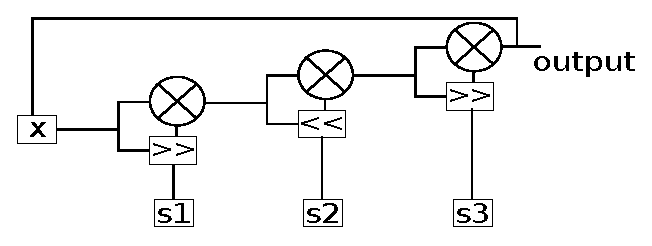
\includegraphics[width=6.5cm]{xorshift.eps}
  \label{xorshift verilog}}
  \subfigure[BBS]{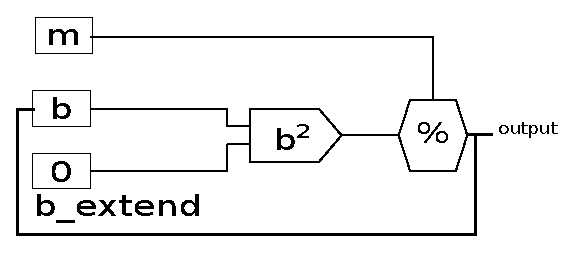
\includegraphics[width=6.5cm]{bbs.eps}
  \label{BBS verilog}}
  \subfigure[The proposed CIPRNG]{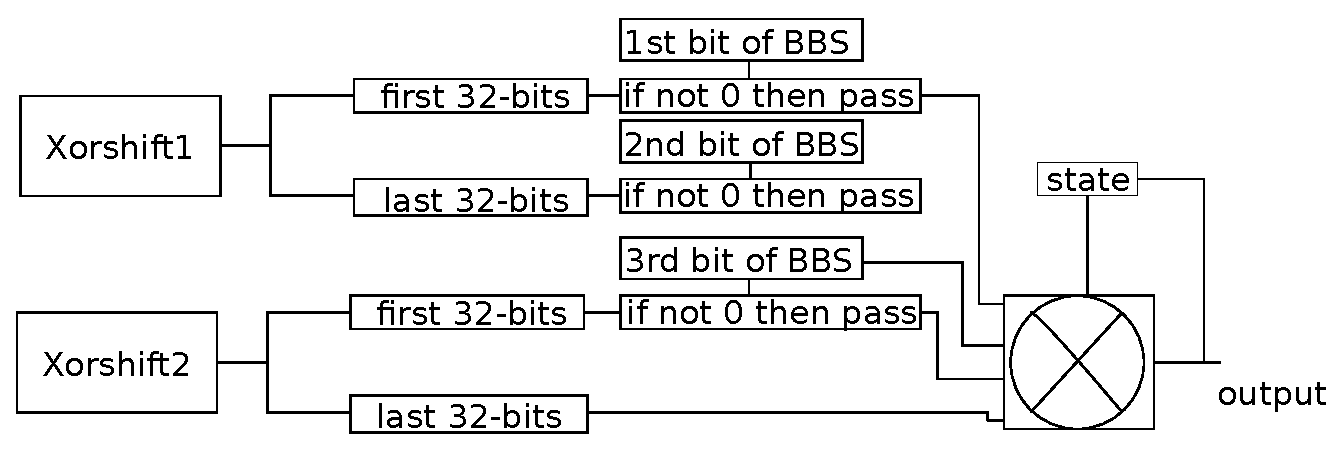
\includegraphics[width=10cm]{ci.eps}
  \label{CI verilog}}
\end{center}
\caption{The processing structure for BBS in FPGA (per clock step)}
\end{figure}
%In our program, we define 
%each FPGA clock positive edge, the XORshift will work, since these are simple processing for FPGA, every 
%clock step can lead to one output.

\subsubsection{Design of BBS}
Fig.\ref{BBS verilog} gives the proposed design of the BBS generator in FPGAs.
There are two inputs of $32$ bits, namely 
$b$ and $m$. 
Register $b$ stores the state of the system
at each time (after the square computation). 
$m$ is also a register that saves the value of $M$, which must not change.
Another register $b\_extend$ 
is used to combine $b$ to a data having $64$ bits, with a view to avoid overflow. 
After the last computation,
the three LSBs from the output of $\%$ are
taken as output. 
Let us notice that a BBS is
 performed at each time unit.

\begin{figure}
\begin{center}
  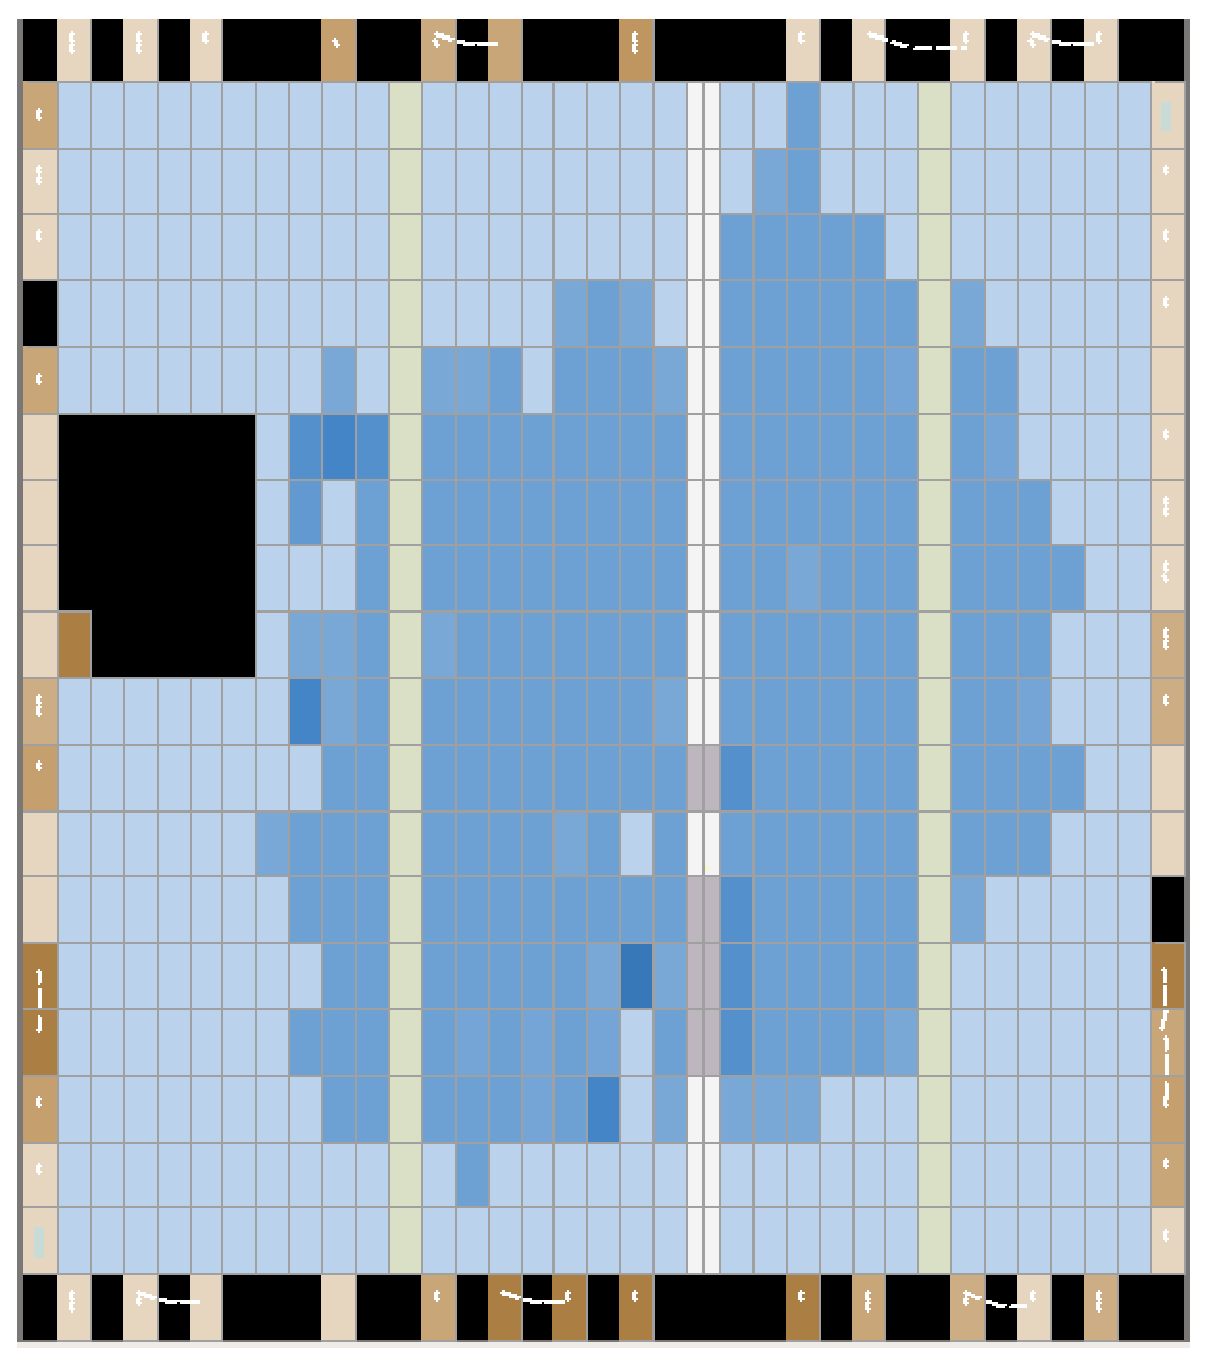
\includegraphics[width=6.5cm]{print.eps}
\end{center}
\caption{The sources cost in $EP2C8Q208C8$ FPGA board}
 \label{logic elements}
\end{figure}

\subsubsection{Design of the chaotic iterations}
Two XORshifts and one BBS are connected to work together, in order to compose the
proposed CIPRNG (see Fig.\ref{CI verilog}). 
As it can be shown, the three bits of the BBS output are switches for the corresponding $32$ bits XORshift outputs. Every round of the 
 processing costs two time units
 to be performed: in the first clock, 
the four PRNGs are processed in parallel,
whereas in the second one, the results of these generators are combined with 
the current state of the system, in order to produce the output of $32$ bits. The output sequence will be appended as Fig.~\ref{ci_OUTPUT} shown, started from the second clock (first clock BBS and XORshift use to initial the first output of CIPRNG).

\begin{figure}
\begin{center}
  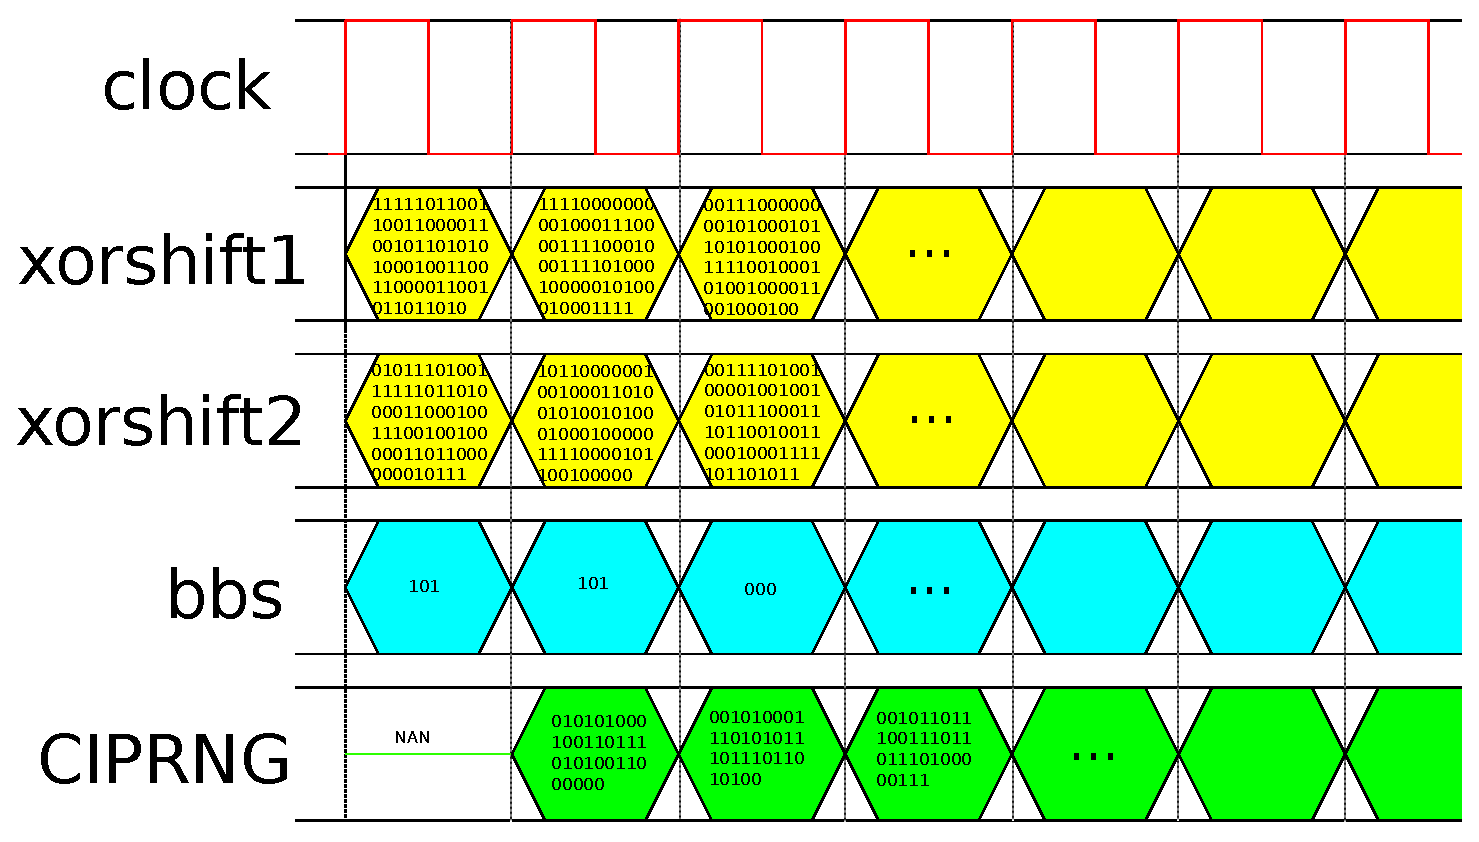
\includegraphics[width=14cm]{ci_OUTPUT.eps}
\end{center}
\caption{Working flow of each component for CIPRNG in FPGA}
 \label{ci_OUTPUT}
\end{figure}

In our experiments, the type $EP2C8Q208C8$ from Altera 
company's CYCLONE II FPGA series 
has been used. By default, its working
frequency is equal to $50$ MHz.
However, it is possible to increase it until
$200$ MHz by using the phase-lock loop (PLL) device.
In that situation, the CIPRNG designed on this
FPGA can produce about $6400$ Mbits per second
(that is, $200 (MHz) \times 32 (bits)$),
while using $3358$ of the $8256$ logic 
elements in $EP2C8Q208C8$ (see
Fig.\ref{logic elements}). 

In Chapter~\ref{Application Example}, an application of this 
CSPRNG designed on FPGA in the information 
hiding security fields is detailed, to show
that this hardware pseudorandom generator 
is ready to use.
